\vspace{-1em}
\section{Introduction}

The nature of data is changing, driven by growing applications such as IoT and monitoring as well as an increasing desire to relate data that spans multiple administrative domains. As a result, data today is {\em heterogeneous}---it spans many different schemas---and {\em evolving}---its schemas change frequently and sometimes unexpectedly. This data with diverse and dynamic schemas---that is, {\em eclectic data}---raises new challenges with ingesting, storing, and querying data. 
In particular, with eclectic data, the process of data discovery becomes a crucial part of the processing pipeline. When data does not conform to a small and well-known set of schemas, then the first step to processing the data is to understand the ``structure’’ of a given data set: discovering what schemas are present, how often each occurs, how similar or dissimilar particular schemas are, and so forth. We use the term {\em data introspection} to refer to this process of exploring the structure of a dataset. Only once users understand the structure of their data can they take steps to transform, clean, or otherwise ``prepare’’ the data for additional processing. In total these steps —  spanning introspection and preparation — can be extremely time consuming, taking 80\% or more of analysts' time~\cite{civilizer}. 
%For example, before a user can query a dataset, they must perform {\em data introspection} to discover what kinds of data it contains (what schemas, how often each occurs, etc.). Once they know what schemas are present, users might also want to transform or clean the data into a smaller set of known schemas. In total these steps to prepare eclectic data for analysis can be extremely time consuming, taking 80\% or more of analysts' time~\cite{civilizer}.

%users need to query across data with heterogeneous and unknown schemas and8 perform {\em data introspection}, by which we mean querying to discover what kinds of data exist in a dataset (what schemas, how often each occurs, etc.). \notesf{mention 80/20 rule somewhere?}

The databases community has long recognized this shift toward eclectic data and, over the last two decades, has vigorously debated different approaches to representing and processing diverse data~\shortorlongform{\cite{what_goes_around, redbook}}{\cite{what_goes_around, redbook_intro}}. Today, the community has largely converged on two data models, which are known to have different strengths and weaknesses. The {\em relational model's} rigid structuring of data according to explicit schemas~\shortorlongform{}{\cite{codd_data_banks, codd_1990}} enables efficient querying and formats such as columnar~\shortorlongform{\cite{dremel, cstore}}{\cite{dremel, cstore, column_vs_row}} as well as data introspection~\cite{aurum} \sr{don't we want to say that the need for sophisticated data introspection and preparation is greatly diminished in this model? if so, move ref to aurum elsewhere}. It is the model of choice for analytics in relational databases\shortorlongform{}{~\cite{postgres, sqlite, sql_server, oracle}} and nested variants of it~\cite{avro, parquet, dremel} form the foundation of big data systems~\cite{spark, hadoop, delta_lake}. However, ingesting heterogeneous and evolving data is not easily supported in the relational model. On the other hand, the {\em document model's} self-describing data values make it trivial to mix heterogeneous data and to ingest data with never-before-seen schemas. Thus data sources commonly generate data in the document model (e.g., JSON), and document databases leverage this model to enable easy ingestion and querying of eclectic data~\cite{mongo, couchbase}. However, this approach sacrifices efficiency and clarity about what kind of data is present. 

It is well-recognized that neither approach is always best, with each of the relational and document models providing functionality that the other lacks. As a result, several recent research efforts and industrial deployments attempt to combine these two and achieve the best of both. For example, some approaches such as AsterixDB can be configured to behave like either the relational model or the document model~\cite{asterixdb, sql++}, while others such as Snowflake or Lakehouses can store some data in each model~\cite{snowflake, postgres, bigdawg, dbms+, delta_lake, lakehouse}.

Unfortunately, as we will discuss (\S\ref{s:hybrid}), even these combined approaches are far from ideal. First, users must contend with two data models: they must decide how to split or replicate their data across both models and a single query can typically leverage the benefits of only one model or the other. Second, to achieve the benefits of explicit schemas (efficient analytics, easy data introspection), users still have to clean their data from the document into the relational model. This cleaning process is known to be complex and brittle~\cite{civilizer, databricks_json_data_ingest}, especially without effective introspection tools to discover what kinds of data are present in the first place. And yet, thirdly, these systems do not make introspection over document data any easier. Thus users are stuck in a catch-22: in order to clean data they must be able to introspect over it, yet in today's systems, rich introspection is only possible after the data has been cleaned.

%Second, in order to benefit from well-defined schemas, users still have to clean their data into the relational model, typically inferring schemas from schemaless data. This process is complex for heterogeneous data and brittle for evolving data, and is part of what led users away from the relational model in the first place. Finally, no existing approach---whether relational, document, or hybrid---provides convenient support for introspecting, querying, or shaping data by its schema.

%\sr{The above para doesn't entirely do it for me. Feels like it doesn't convey the importance of introspection.  How about the following (borrowing from your outline):\\
%Unfortunately, as we will show (\S\ref{s:hybrid}), even these hybrid approaches are far from ideal. First, users must continue to contend with two data models: they must decide how to split or replicate their data across both models and a single query can leverage the benefits of only one model or the other. Second, to acheive the benefits of well-defined schemas (efficient analytics, easy data introspection), users still have to clean their data from the document into the relational model. This cleaning process is known to be complex and brittle~\cite{80,20} but these hybrid systems do nothing to resolve the catch-22 situation that makes cleaning inherently challenging: i.e., that in order to clean data we must be able to introspect over it (define introspection earlier — discover what types of records exist, the frequency of each, “shape” of data, etc); yet, in today’s systems, rich introspection is only possible after the data has been cleaned.}

% \notesf{I wonder if this paragraph right below should come earlier/before the previous paragraph?}
We believe that these approaches fall short because they are {\em hybrid} rather than truly {\em unified}. They co-implement both data models and require a shim layer on top. This is complex and brittle, and for a given piece of data, you can only reap the benefits of one model at a time. Taking a step back, we wondered if this sacrifice is truly necessary, or if perhaps a solution could be found by addressing the problem at a lower layer. Perhaps it is time, yet again, to rethink the foundations of data processing: the data model and query language.

We argue that eclectic data would benefit from a {\em new approach to unification} in which a single data model and query language can simultaneously provide the benefits of both explicit schemas (efficient analytics, ease of introspection) and mixed heterogeneous data (seamless ingestion).% In addition, this model must provide comprehensive support for data introspection.

We start with the observation that what fundamentally enables both efficient analytics and data introspection is knowing the {\em type} of each piece of data. For example, this allows us to store data in formats that are organized by type (e.g., by column) and to query for information about what types of data are present. The relational model has this explicit type information, but is overly rigid in how it uses it, only accepting data from a pre-defined set of schemas. Attempts to relax this rigidity by conveying new schemas via schema registries~\cite{confluent_schema_registry} still don't enable query results to flexibly mix heterogeneous data \sr{I don't see this as the main problem with schema registries! I'd go back to the text in my comment below.}. This leads us to the goal of {\em comprehensive yet flexible typing}\notesf{this feels like the desired property of the data model; the original text ``This leads us to the goal of defining a data model in which all data is typed but that doesn't constrain what types are permitted'' feels better to me, although I understand that you really want to focus on ``type'' here. But honestly, I feel the story could be smoother (..I could be very wrong) to have a focus on data model and then dive into type (as the data model's novel design), which I think would've engaged the audience better to rethink about data model. See the comment at the end of intro.}. By this we mean that every data value has an explicit, queryable type (i.e., users can query for or by type), and yet there are no constraints on which types are permitted to coexist (e.g., in the same file, table, or set of query results). Furthermore, this data and its type information should be self-contained so that parsing data never requires coordination with an external registry. \sr{it's more than just this? self-contained also gives us the nice property that one can query type information in exactly the same way - same language, store, etc - as one queries the data? And that this simplifies data introspection?}

%\sr{Needs some connecting tissue here to lead the reader to types as the answer? Can we say something like: We start with the observation that what fundamentally enables both efficient analytics and data introspection is knowing the \emph{type} of data we have. Having type information allows us to, for example, use formats that organize data by type (e.g., by column) for efficent processing, and allows us to reason about the shape of data available (e.g., how many types exist, how many records of each type). The relational model has the well-defined type information that we seek but the problem is it’s overly rigid in its use of this type information — only accepting data from a pre-defined set of types. And attempts to relax this rigidity have introduced new problems — e.g., they add new external components (e.g., schema registries) that require complex integrations with the storage and query processing components, or they resort to weakly defined types (e.g., object) that can’t fully utilize the benefits of types. This leads us to the goal of defining a data model in which all data is typed but that doesn’t constrain what types are permitted. Moreover, this data together with its type information should be self-contained - i.e., the data model must capture both data and their type information in one coherent architecture. These observations lead us to a new data model in which \ldots.} 
%Our unified approach begins with two goals, centered around {\em data types}. First, every data value should have an explicit, queryable type. This enables efficient storage and querying, avoids error-prone schema inference, and enables queries about data types, such as introspection and shaping. At the same time, we should be flexible about which data types are allowed to coexist in the same file, table, or set of query results.
%\noteamy{need to rework the previous 2 paragraphs. they focus too much on limitation 1 and don't really cover 2 or 3.}

%\notesf{I don't find the key idea come through crisply from the current text in the two paragraphs below and I think we should mention schema registries. Let's discuss?}

\begin{figure*}[t]
    \centering
    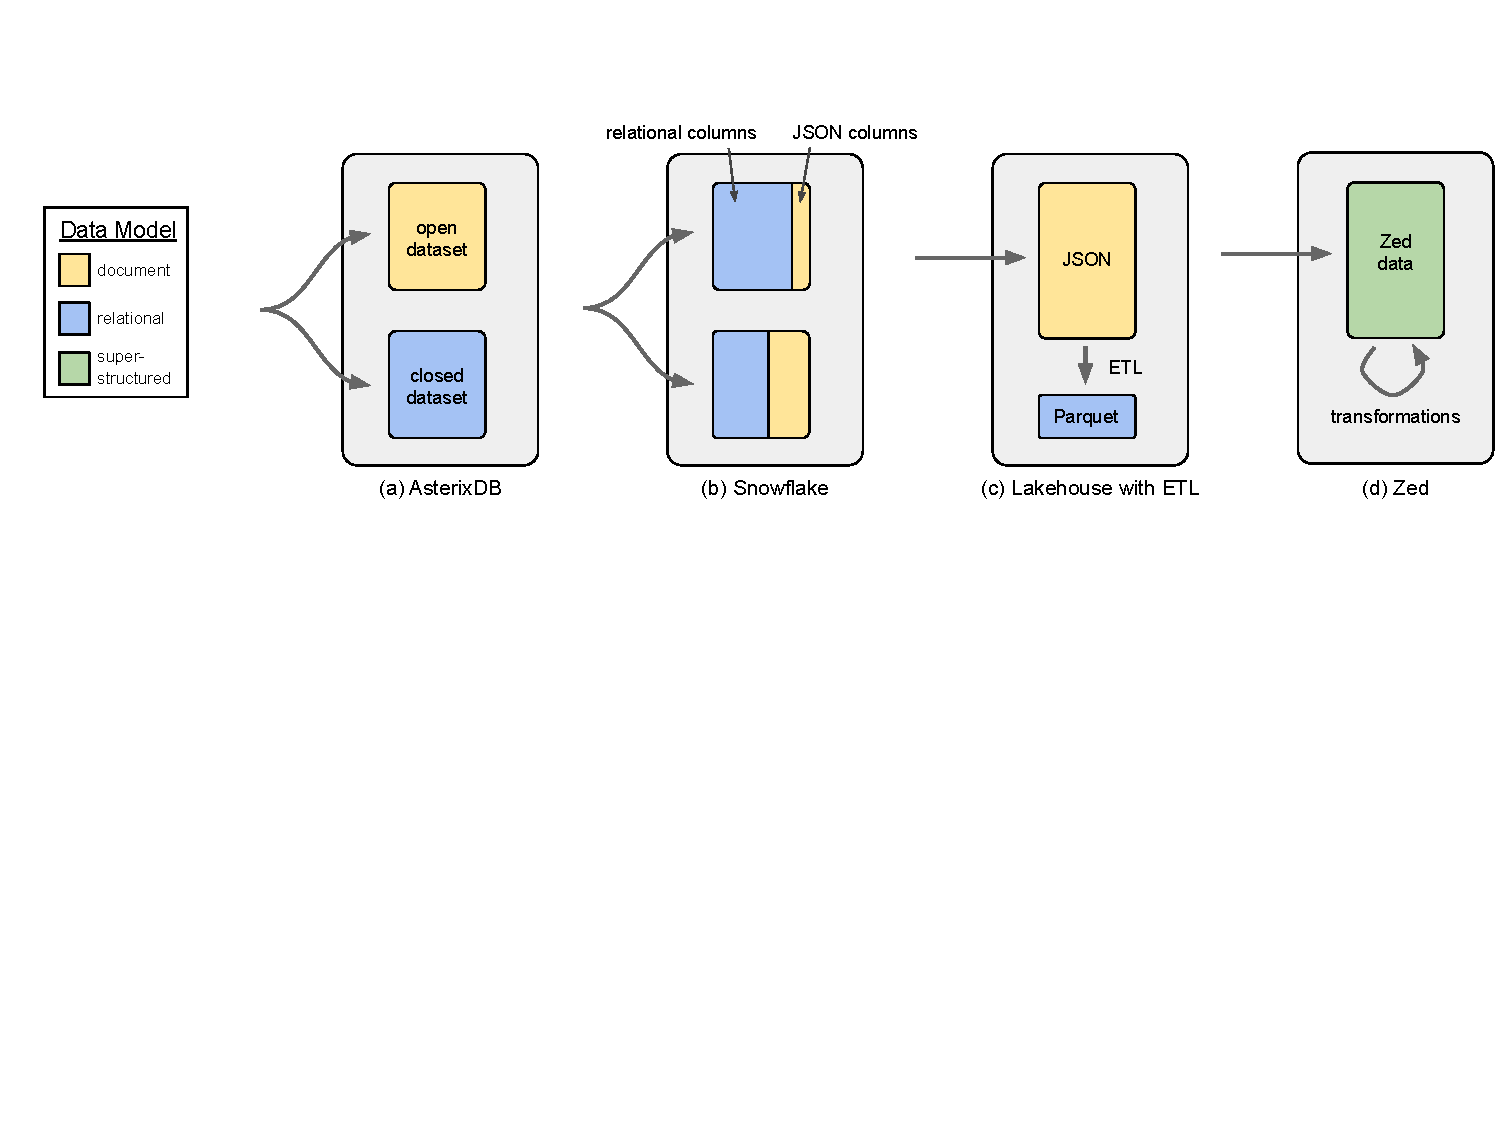
\includegraphics[width=0.85\textwidth]{figures/hybrid_approaches.pdf}
    \vspace{-1em}
    \caption{Three example hybrid approaches to data processing: (a) AsterixDB splits incoming data into open and closed datasets in separate files, (b) Snowflake adds columns of JSON data to each relational table, and (c) Lakehouses use ETL to clean a subset of JSON data into Parquet. (d) In Zed, all data (raw or transformed) is represented in the super-structured data model.}
    \label{f:hybrid_approaches}
    \vspace{-1em}
\end{figure*}

The key to achieving comprehensive yet flexible typing is to change the way that we associate type information with data values. Instead of associating a single schema with each file or table, which makes it difficult to store or process heterogeneous data together, we propose a new {\em data type abstraction} that is associated directly with individual data values. This enables each value to have an explicit data type (as in the relational model) but also allows different values that are processed together to have different types (as in the document model). We call the resulting data model the {\bf super-structured data model}, because it subsumes the structures of the relational and document data models. Data is organized as a sequence of typed values; when all values have the same type, this model is equivalent to the relational model.

%\sr{Elaborate? I.e., data is ingested as an ordered stream of typed values. And when all data are the same type, the super-structured model is equivalent to the relational model}\notesf{I strongly agree; I find this a key observation.} 

% \notesf{summarize this by saying ``deep typing without schema rigidity''?} \noteamy{I'm not sure that ``deep typing without schema rigidity'' quite captures the key properties of \sys{}. If we want a summary at that level of detail, what about: ``type flexibility and first-class types''?}

Realizing this approach requires care in designing the type abstraction. We propose an abstraction with the following properties:
\begin{CompactItemize}
    \item Types are {\em associated with individual values}, rather than with a collection such as a table or file.
    \item Types are {\em complete} - we observe that catch-all types such as ``object'' or ``json'', or allowing a value to include extra fields beyond those specified by its type prevent the full benefits of types.
    \item Types are {\em first class} - users can query for data types and the query results---which contains types---are returned in the same data model. Users can refer to types by name and data formats can assign numeric type IDs for efficient storage and querying.
    %\item Data types should be {\em identifiable} (i.e., types can be referred to by a numeric ID or string name) - this enables efficient storage and querying because data values can be tagged with their numeric type. It also enables querying values by their type, e.g., to extract all values with a given type, effectively extracting a single relational table from heterogeneous data.
    \item Type definitions are {\em inlined} - this enables data sources to define new types on the fly without out-of-band coordination or additional burden relative to writing JSON data.
\end{CompactItemize}

In this paper we propose {\bf \sys{}}, a new approach to data processing that is centered around these data types. \sys{} includes a new super-structured data model (\S\ref{ss:zed_data_model}) and query language (\S\ref{ss:zed_query_language}). In addition, \sys{}'s type abstraction allows data to be represented in the format most suitable for the task at hand: columnar for analytics, human-readable for debugging, etc.  Because all data is typed, converting it between formats within the family is lossless and fully automated. Thus \sys{} includes a ``family of data formats'' (\S\ref{ss:zed_formats}). Finally, we will show how \sys{} overcomes the challenges of existing hybrid approaches and unifies the document and relational models in a new way, {\em embodying both at the same time}  (\S\ref{s:zed_in_action}). %\sys{} enables: easy data generation and ingestion, with the ability to create new types on the fly; efficient storage and analytics; data introspection at any stage of data processing; and simplicity, with no dependency on external components such as schema registries (\S\ref{s:zed_in_action}).
\notesf{The story in its current form focuses on ``eclectic data'' -> ``first-class type in query language and data model'' which makes sense, but the key message/nugget ``a new data model that has comprehensive type and no rigid schema can do both what relational model and document model can do, yet without schema registry's operational overhead'' is somewhat nebulous. But perhaps that has been the presentation challenge/struggle, a trade-off difficult to make right.}
\noteamy{I think the query language part is crucial to the story though, so I think our main pitch needs to be broad enough to include both the data model and query language. For example, if the query language didn't support queries like typeof(this)==<x>, then Zed wouldn't subsume the relational model because you wouldn't be able to extract all records with a give type. Maybe the importance of the query language needs to come through more clearly?}\notesf{I don't disagree on the importance of query lang at all and that part comes through in the design section well (I'm less sure on the intro). I was more referring to the ``nugget'' bits in my comment. Do you find that nugget come through well? :)}

\notesf{actually, perhaps this is where our views diverge: the current story leads with ``type'', then say how ``query lang'' and ``data model'' support the first-class type; whereas in the ``nugget'' above it was the opposite: lead with the ``data model'' and then say how to implement the data model with ``comprehensive type and no rigidity''. Honestly, for me, I'm fine with either case, esp. given the time left and that I didn't realize/bring this up earlier, although I still find the latter works for me better (I'd think it's also the flow on Steve's blog?); I find it flow smoother with the rethink relational model/document model -> unified model -> comprehensive type with no rigidity -> type context -> family formats -> query language.}

%and unification of the document and relational models subsuming both with a single instantiation of data 

%Finally, we will conclude with a discussion and directions for future research (\S\ref{s:conclude}).